%----------------------------------------------------------------------------------------
%	Inställningar och dokumentkonfiguration
%----------------------------------------------------------------------------------------

\documentclass[paper=a4, fontsize=11pt]{report} % A4-sida och 11 punkters fontstorlek

\usepackage[T1]{fontenc} % 8-bitarskodning som har 256 glyfer
\usepackage[english]{babel} % Svenskt språk
\usepackage[utf8]{inputenc} % För svenska tecken
\usepackage{dtklogos} % Logos
\usepackage{wallpaper} % Bakgrundsbild
\usepackage{fancyhdr} % Specialsidhuvud och sidfot
\usepackage{enumerate} 
\usepackage{xifthen}% provides \isempty test
\usepackage{listings}% Code examples
\usepackage{xcolor}
\newcounter{tmpc}
\lstdefinestyle{BashInputStyle}{
  language=bash,
  basicstyle=\footnotesize\ttfamily,
  numbers=left,
  numberstyle=\tiny,
  numbersep=3pt,
  frame=tb,
  columns=fullflexible,
  backgroundcolor=\color{yellow!20},
  linewidth=0.9\linewidth,
  xleftmargin=0.1\linewidth
}
% Exampels
% Inline
% \lstinline[style=BashInputStyle]´# apt-get --purge remove rubygems´.
% Multiline
% \begin{lstlisting}[style=BashInputStyle]
%    # apt-get --purge remove rubygems
% \end{lstlisting}

\pagestyle{fancyplain} % Använd sidhuvud och sidfot på alla sidor
\fancyhead[L]{Seminar 5 -- 1DV020 -- 2015 -- Server Administration} % Titel till vänster i sidhuvud
\fancyhead[C]{} % Tomt i mitten
\fancyhead[R]{} % Tomt till höger
\fancyfoot[L]{} % Tomt till vänster
\fancyfoot[C]{} % Tomt i mitten
\fancyfoot[R]{\thepage} % Sidnumrering till höger i sidfoten
\renewcommand\thesection{\arabic{section}} % Section beter sig som i dokumentklassen article

\newcommand{\win}[1]{Microsoft Windows Server\ifthenelse{\isempty{#1}}{}{ #1}}
\newcommand{\gui}[0]{``Server with a GUI''}
\newcommand{\core}[0]{Windows Server Core}
%----------------------------------------------------------------------------------------
%	TITLE SECTION
%----------------------------------------------------------------------------------------
\newcommand\BackgroundPic{
    \put(-50,-50){
    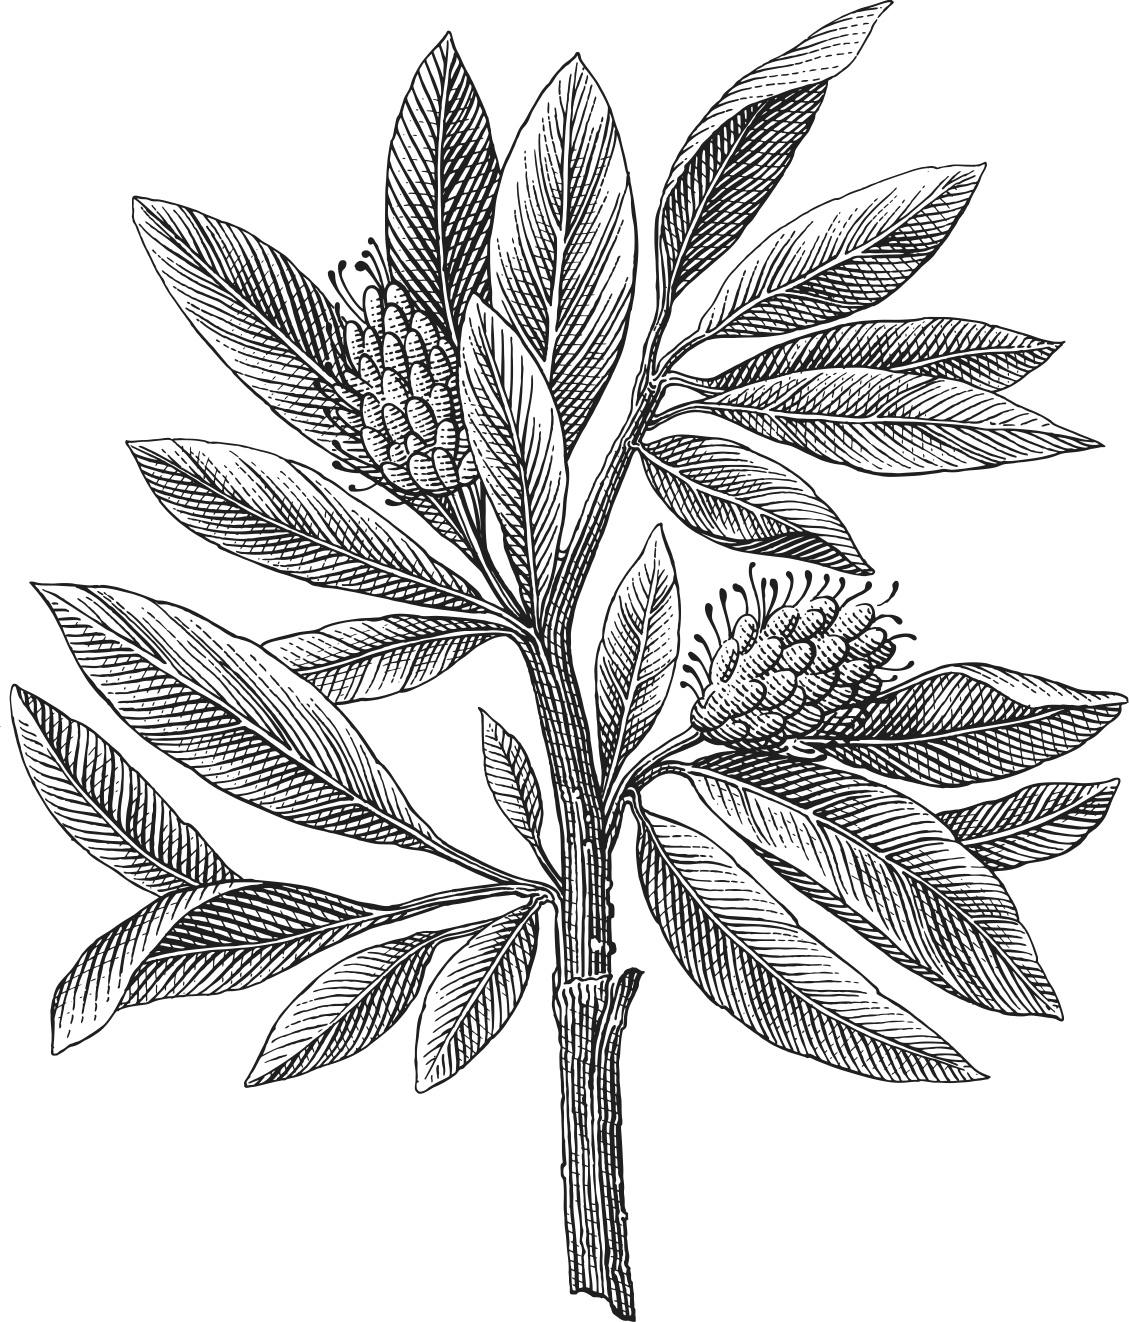
\includegraphics[keepaspectratio,scale=0.65]{lnu_etch.png} % Bakgrundsbild
    }
}
\newcommand\BackgroundPicLogo{
    \put(15,700){
    
\includegraphics[keepaspectratio,scale=0.10]{logo.png} % Logga i vänstra hörnet
    }
}

\newcommand{\horrule}[1]{\rule{\linewidth}{#1}} % Skapa hortisontell linje

\title{	\vspace{-10cm}
    \normalfont \normalsize
    \textsc{Linnaeus University} \\ [25pt] % Universitetes namn
    \horrule{0.5pt} \\[0.4cm] % Tunn linje högst upp
    \huge Seminar 5\\ % Arbetes titel
	\large \textcolor{gray}{1DV020 -- Server Administration}
    \horrule{0.5pt} \\[0.4cm] % Tunn linje längst ner
}

\author{Jacob Lindehoff} % Författarnas namn

\date{\normalsize\today} % Dagens datum

\begin{document}
\AddToShipoutPicture*{\BackgroundPic} % Lägger in backgrundsbild på första sidan
\AddToShipoutPicture*{\BackgroundPicLogo}
\maketitle % Skriv ut titeln
\noindent % Tabba inte in på första meningen


%------------------------------------------------
%	Introduktion
%------------------------------------------------
\section{Introduction}
During this seminar, we will address the following topics:
\begin{itemize}
\item Skriptning
\begin{itemize}
    \item Grunderna
    \item Användbara kommandon
    \item Jobba mot Active Directory
    \item Batch skript
\end{itemize}
\item Backup
\item Volume Shadow Copy
\item Diskhantering
\item Skriptning
\begin{itemize}
    \item Performance Monitor
    \item Event Viewer
\end{itemize}
\end{itemize}

%------------------------------------------------
%	Deadline
%------------------------------------------------
\section{Dealine}
  The seminar is on the {\color{red}11th of March 2015} and it is compulsory. If you cannot participate, it must be notified in advance and a written report of the seminar must be submitted no later than {\color{red}3 days} after the seminar. The written report should contain detailed answers to all questions in the seminar.\newpage
%------------------------------------------------
%	Seminariefrågor
%------------------------------------------------
\section{Seminariefrågor}
\begin{enumerate}
\begin{large}
\item Förklara hur man navigerar i kommandoprompten och vilka kortkommandon som är bara att känna till.
\item Förklara vad följande kommandon används till. Om det finns tilläggsväxlar till kommandona så beskriv även hur dessa används.
\begin{enumerate}[a.]
	\item cls
	\item dir
	\item type
	\item mkdir
	\item rmdir
	\item cd
	\item del
	\item xcopy
	\item move
	\item rename
	\item net share
	\item net use
	\item net start
	\item dsadd
	\item dsget
	\item dsquery
\end{enumerate}
\item Vad är ett ''Distinguished Name''?
\item Vad gör följande kommando:
dsquery user ''OU=Users, OU=Washington, DC=mediawork, DC=local'' | dsmod user -desc ''Washington User''
\item Hur fungerar skriptfiler?
\item Hur använder man sig av variabler i skript?
\item Det kan ofta bli problem med svenska tecken som åäö i skriptfiler, vad beror detta på och hur löser man detta?
\item Hur gör man för att flytta runt exekveringen i en skriptfil?
\item Beskriv hur de fyra olika FOR-looparna fungerar?
\item Beskriv följande typer av backup:
\begin{enumerate}[a.]
	\item Full eller Normal backup
	\item Differential backup
	\item Incremental backup
\end{enumerate}
\item Hur fungerar Windows Server Backup i Windows Server 2012 R2?
\item Vad är Volyme Shadow Copy och hur fungerar det?
\item Vilka verktyg finns integrerade i operativsystem för att hantera felsökning och övervakning i Windows Server?
\end{large}
\end{enumerate}
\end{document}
